Интерфейс предполагает вывод первых 10 элементов из 1000 каждой последовательности (за исключением той, которую введёт пользователь, так как в этом случае длина фиксирована и равна 10). 

Результат работы программы приведен на рисунке \ref{fig1:image}. Можно заметить, что значения критерия в любом из столбцов находится в интервале от 0.1 до 0.9, что позволяет считать последовательности случайными.

\begin{figure}[h]
	\begin{center}
		{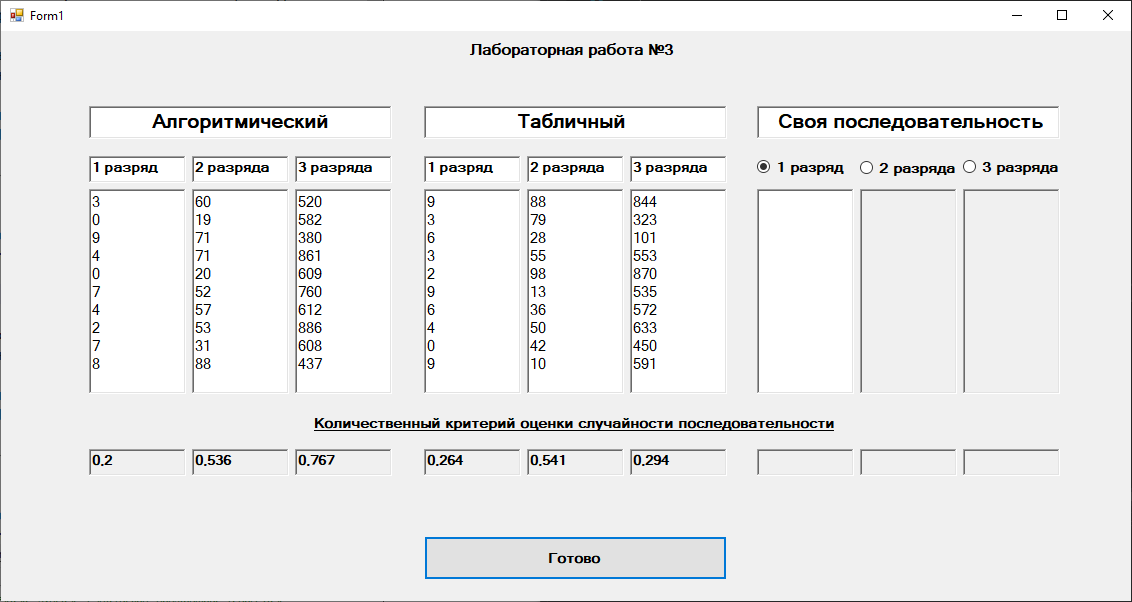
\includegraphics[scale = 0.55]{img/ex1.png}}
		\caption{Пример 1}
		\label{fig1:image}
	\end{center}
\end{figure}

На рисунках \ref{fig2:image}-\ref{fig4:image} демонстрируются примеры пользовательских последовательностей.

\begin{figure}[h]
	\begin{center}
		{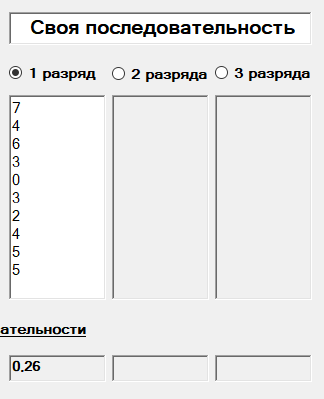
\includegraphics[scale = 0.55]{img/ex4.png}}
		\caption{Пример 2. Введенная пользователем последовательность из 10 чисел}
		\label{fig2:image}
	\end{center}
\end{figure}

\begin{figure}[h]
	\begin{center}
		{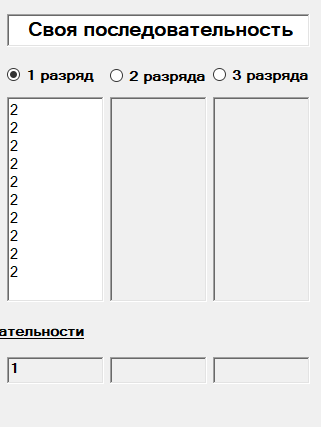
\includegraphics[scale = 0.55]{img/ex2.png}}
		\caption{Пример 3. Все числа одинаковые}
		\label{fig3:image}
	\end{center}
\end{figure}

\begin{figure}[h]
	\begin{center}
		{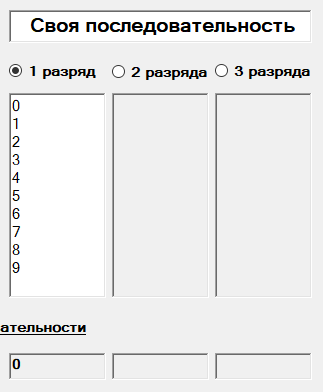
\includegraphics[scale = 0.55]{img/ex3.png}}
		\caption{Пример 4. Подряд идущие числа}
		\label{fig4:image}
	\end{center}
\end{figure}

